\documentclass{article} % For LaTeX2e
\usepackage{iclr2016_conference,times}
\usepackage{hyperref}
\usepackage{url}
\usepackage{algorithm,algorithmic}
\usepackage{amsmath}
\usepackage{amssymb}
\usepackage{graphicx}
\usepackage{caption}
\usepackage{subcaption}
\usepackage{amsthm}
\usepackage{bbm}
\usepackage{booktabs}
\usepackage{array,multirow}
%\usepackage[table,xcdraw]{xcolor}
%\documentstyle[nips13submit_09,times,art10]{article} % For LaTeX 2.09

\newcommand{\argmin}{\operatornamewithlimits{argmin}}


\title{Infinite Dimensional Word Embeddings}


\author{Eric T. Nalisnick \thanks{ Authors contributed equally.} \\
Department of Computer Science\\
University of California, Irvine\\
Irvine, CA 92697, USA \\
\texttt{enalisni@uci.edu} \\
\And
Sachin Ravi $^{*}$\\
Department of Computer Science \\
Princeton University \\
Princeton, NJ 08540, USA \\
\texttt{sachinr@cs.princeton.edu} 
}

% The \author macro works with any number of authors. There are two commands
% used to separate the names and addresses of multiple authors: \And and \AND.
%
% Using \And between authors leaves it to \LaTeX{} to determine where to break
% the lines. Using \AND forces a linebreak at that point. So, if \LaTeX{}
% puts 3 of 4 authors names on the first line, and the last on the second
% line, try using \AND instead of \And before the third author name.

\newcommand{\fix}{\marginpar{FIX}}
\newcommand{\new}{\marginpar{NEW}}

%\iclrfinalcopy % Uncomment for camera-ready version

\begin{document}


\maketitle

\begin{abstract}
We describe a method for learning word embeddings with stochastic dimensionality. Our \textit{Infinite Skip-Gram} (iSG) model specifies an energy-based joint distribution over a word vector, a context vector, and their dimensionality.  By employing the same techniques used to make the Infinite Restricted Boltzmann Machine \citep{cote2015infinite} tractable, we define vector dimensionality over a countably infinite domain, allowing representations to grow as needed during training.  After training, we find that the distribution over embedding dimensionalities for a given word is highly interpretable and leads to an elegant probabilistic mechanism for word sense induction. We show qualitatively and quantitatively that the iSG produces parameter-efficient representations that are robust to language's inherent ambiguity.
\end{abstract}

\section{Introduction}
\textit{Neural language modeling} (NLM) \citep{bengio2003neural, mnih2009scalable, turian2010word, mikolov2013distributed} has received wide-spread attention for its ability to capture surprisingly detailed semantic information without supervision.  NLM is built off the key idea that the \textit{distributional hypothesis} \citep{harris1954distributional} can be formulated as a prediction task: for a given word, predict its neighboring words (or vice versa).  After training a classifier in this way, a \textit{distributed representation} for each word token can be found in the model parameters.  These high-dimensional, real-valued vectors--called \textit{(Neural) Word Embeddings} (WEs)--have been shown to be experimentally superior to discrete representations \citep{baroni2014don} (ostensibly) due to their ability to capture semantic subtlety and withstand ambiguity.

However, despite their success, WEs still have deficiencies.  One flaw is that the vectors, since their dimensionality is fixed across the vocabulary, do not accurately reflect each word's semantic complexity.  For instance, the meaning of the word \textit{race} varies with context (ex: car race vs biological race), but the meaning of \textit{regatta} is rather specific and invariant.  It seems unlikely that \textit{race} and \textit{regatta}'s representations could contain the same number of parameters without one overfitting or underfitting.  

To better capture the semantic variability of words, we propose a novel embedding method that produces vectors with stochastic dimensionality.  By employing the same mathematical tools that allow the definition of an \textit{Infinite Restricted Boltzmann Machine} \citep{cote2015infinite}, we describe a log-bilinear energy-based model--called \textit{Infinite Skip-Gram} (iSG)--that defines a joint distribution over a word vector, a context vector, and their dimensionality, which has a countably infinite domain.  During training, the iSG allows word representations to grow naturally based on how well they can predict their context.  This behavior enables the vectors of specific words to use few dimensions and the vectors of vague words to elongate as needed.  Manual and experimental analysis reveals this dynamic representation elegantly captures specificity, \textit{polysemy}, and \textit{homonymy} without explicit definition of such concepts within the model.  As far as we are aware, this is the first word embedding method that allows representation dimensionality to be variable and exhibit data-dependent growth\footnote{\cite{bartunov2015breaking} proposes an infinite dimensional model based on Bayesian Nonparametrics (which will be reviewed in Section \ref{related}), but their model specifies an infinite number of independent, fix-sized vectors per word.}.

\section{Original Skip-Gram}
We first review the original \textit{Skip-Gram} architecture before describing our novel, infinite-dimensional extension in Section \ref{isgm_sec}.  \textit{Skip-Gram} (SG) (along with its sister model \textit{Continuous Bag-of-Words} (CBOW)) is arguably the most popular method for learning word embeddings \citep{mikolov2013distributed}\footnote{The software \textit{Word2Vec} provides a fast, multi-threaded implementation of both SG and CBOW: https://code.google.com/p/word2vec/}.  Its widespread use is probably due to its simplicity.  SG is a computationally lean log-bilinear model whereas most previous neural language modeling had been done with neural networks.     

SG learns a word's embedding via maximizing the log probability of that word's context (i.e. the words occurring within a fixed-sized window around the input word).  Formally, let $\mathbf{w}_{i} \in \mathbb{R}^{d}$ be a $d$-dimensional, real-valued vector representing the $i$th input word $w_{i}$, and let $\mathbf{c}_{k} \in \mathbb{R}^{d}$ be a vector representing the $k$th context word $c_{k}$ appearing in a $2K$-sized window around an instance of $w_{i}$ in some training corpus $\mathcal{D}$.  Training the SG model reduces to minimizing the following objective function: \begin{equation}\begin{split}\label{sg_def} \mathcal{L}_{SG} &= \sum_{i=1}^{|\mathcal{D}|} \sum_{i-K\le k \le i+K, k\ne i} - \log p(c_{k} | w_{i}) \\ &= \sum_{i=1}^{|\mathcal{D}|} \sum_{i-K\le k \le i+K, k\ne i} - \log \frac{e^{\mathbf{c}_{k}^{T}\mathbf{w}_{i}}}{\sum_{v=1}^{V_{c}} e^{\mathbf{c}_{v}^{T}\mathbf{w}_{i}}} \\ &= \sum_{i=1}^{|\mathcal{D}|} \sum_{i-K\le k \le i+K, k\ne i} - \mathbf{c}_{k}^{T}\mathbf{w}_{i} + \log \sum_{v=1}^{V_{c}} e^{\mathbf{c}_{v}^{T}\mathbf{w}_{i}} \end{split}\end{equation} where $V_{c}$ is the size of the context vocabulary.  Stochastic gradient descent is used to update not only $\mathbf{w}_{i}$ but also $\mathbf{c}_{k}$ and $\mathbf{c}_{v}$.  From here forward we drop the summations over the corpus and context window to simplify notation.

Notice the cost of these gradient computations is proportional to $V_{c}$, which is usually several million or more.  A \textit{hierarchical softmax} or \textit{negative sampling} is commonly used to alleviate the computation burden of full normalization \citep{mikolov2013distributed}.  We'll only consider the latter, but all models discussed can be can be adapted straightforwardly to use a hierarchical softmax.  Negative sampling consists of randomly sampling (either from the uniform or empirical distribution) words to serve as negative examples--words that \textit{do not} appear in the current context window--and then optimizing so that the true context word has a higher likelihood than the samples.  Using negative sampling for computing Equation \ref{sg_def} results in the following modification:  \begin{equation}\begin{split}\label{sg_w_neg} - \mathbf{c}_{k}^{T}\mathbf{w}_{i} + \log \sum_{v=1}^{V_{c}} e^{\mathbf{c}_{v}^{T}\mathbf{w}_{i}} \approx -\mathbf{c}_{k}^{T}\mathbf{w}_{i} + \log  \left [ \sum_{s=1}^{S} e^{\mathbf{c}_{s}^{T} \mathbf{w}_{i}} + e^{\mathbf{c}_{k}^{T} \mathbf{w}_{i}} \right ] \end{split}\end{equation} for $S$ negative samples.  Notice that we have defined a slightly different negative sampling SG objective than proposed in \cite{mikolov2013distributed}, which incorporates logistic regression to discriminate the true context word from the samples.  However, other embedding models such as \cite{huang2013learning} have used the negative samples directly in the normalizing sum, as we do.  

\section{Infinite Skip-Gram}\label{isgm_sec}
We now propose our novel modification to the Skip-Gram architecture, which we call the \textit{Infinite Skip-Gram} (iSG) model.  Let word vectors $\mathbf{w}_{i} \in \mathbb{R}^{\infty}$ and context vectors $\mathbf{c}_{k} \in \mathbb{R}^{\infty}$ be infinite dimensional (instead of fixed dimensionality $d$), and redefine the model to be the following joint Gibbs distribution over $\mathbf{w}_{i}$, $\mathbf{c}_{k}$, and a random positive integer $z \in \mathbb{Z}^{+}$ denoting the maximum index over which to compute the vector inner product: \begin{equation}
p(w_{i}, c_{k}, z) = \frac{1}{Z} e^{-E(\mathbf{w}_{i}, \mathbf{c}_{k}, z)} 
\end{equation} where $Z = \sum_{\mathbf{w}} \sum_{\mathbf{c}} \sum_{z} e^{-E(\mathbf{w}, \mathbf{c}, z)}$, also known as the partition function.  Define the energy function as \begin{equation}
E(\mathbf{w}_{i}, \mathbf{c}_{k}, z) = z\log a - \sum_{j=1}^{z} w_{i,j}c_{k,j} - \lambda w_{i,j}^{2} - \lambda c_{k,j}^{2} 
\end{equation} where $1 < a < \infty$, $a \in \mathbb{R}$ and $\lambda$ is a weight on the L2 penalty.  The $\log a$ term may seem superfluous, but, as we'll see in the next section, it is necessary for defining a convergent geometric series and controls the model's growing behavior.  
\subsection{A Finite Partition Function}
At first glance the iSGM seems intractable since the partition function, containing a sum over all countably infinite values of $z$, would seem to be divergent and thus incomputable.  However, it is not, due to two key properties first proposed by \cite{cote2015infinite} to define a \textit{Restricted Boltzmann Machine} with an infinite number of hidden units (iRBM).  They are: \begin{enumerate}
  \item \textbf{Sparsity penalty}: The $L2$ penalty incorporated into $E(\mathbf{w}_{i}, \mathbf{c}_{k}, z)$ (i.e. the $w_{i,j}^{2}$ and $c_{k,j}^{2}$ terms) ensures the word and context vectors must have a finite two-norm.  That is to say all elements of $\mathbf{w}$ and $\mathbf{c}$ at an index greater than or equal to some sufficiently large index $l$ \emph{must be zero}.  No proper optimization method could converge to the infinite solution if all $\mathbf{w}$ and $\mathbf{c}$ vectors are initialized to have a finite number of non-zero elements \citep{cote2015infinite}.
  \item \textbf{Per-dimension constant penalty}:  The energy function's $z\log a$ term results in dimensions greater than $l$ becoming a convergent geometric series.  This is discussed further below and shown in detail in the appendix.  
\end{enumerate}
With those two properties in mind, consider the conditional distribution of $z$ given an input and context word: \begin{equation}
p(z | w, c) = \frac{e^{-E(\mathbf{w}, \mathbf{c}, z)}}{\sum_{z'=1}^{\infty} e^{-E(\mathbf{w}, \mathbf{c}, z')}}. \end{equation}  Again, the denominator looks problematic due to the infinite sum, but notice the following (a detailed derivation is in the appendix): \begin{equation}\begin{split}\label{z_finite}
Z_{z} &= \sum_{z'=1}^{\infty} e^{-E(\mathbf{w}, \mathbf{c}, z')}  = \sum_{z'=1}^{l} e^{-E(\mathbf{w}, \mathbf{c}, z')} + \sum_{z'=l+1}^{\infty} e^{-E(\mathbf{w}, \mathbf{c}, z')} \\ &= \sum_{z'=1}^{l} e^{-E(\mathbf{w}, \mathbf{c}, z')} + e^{-E(\mathbf{w}, \mathbf{c}, l)} \sum_{z'=0}^{\infty} \frac{1}{a^{  z' }} \\ &= \sum_{z'=1}^{l} e^{-E(\mathbf{w}, \mathbf{c}, z')} + \frac{a}{a-1}e^{-E(\mathbf{w}, \mathbf{c}, l)}.
\end{split}
\end{equation}  As stated in other words above, the sparsity penalty allows the sum to be split as it is in step \#2 into a finite term ($\sum_{z'=1}^{l} e^{-E(\mathbf{w}, \mathbf{c}, z')}$) and an infinite sum ($\sum_{z'=l+1}^{\infty} e^{-E(\mathbf{w}, \mathbf{c}, z')}$) at an index $l$ such that $w_{i,j}=c_{k,j}=0$ $\forall j>l$.  After $e^{-E(\mathbf{w}, \mathbf{c}, l)}$ is factored out of the second term, all remaining $w_{i,j}$ and $c_{k,j}$ terms are zero.  A few steps of algebra then reveal the presence of a convergent geometric series.  Intuitively, we can think of the second term, $\frac{a}{a-1}e^{-E(\mathbf{w}, \mathbf{c}, l)}$, as quantifying the data's need to expand the model's capacity given $w$ and $c$.   
\subsection{Learning}\label{learn_isg}
We now turn our attention to learning the iSGM.  We look to treat $z$, the random index variable, as a nuisance parameter and optimize an upper-bound to the traditional Skip-Gram objective:\begin{equation}\begin{split}\label{iSGM_obj}
\mathcal{L}_{SG} &= - \log p(c_{k} | w_{i}) \\ &= - \log \sum_{z=1}^{\infty} p(c_{k}, z| w_{i}) \\ &= - \log \sum_{z=1}^{\infty} p(c_{k}| w_{i}, z) p(z | w_{i}) \\ &\le  \sum_{z=1}^{\infty} p(z | w_{i}) -\log p(c_{k}| w_{i}, z) \\ &= \mathbb{E}_{z|w}[- \log p( c_{k}| w_{i}, z)] = \mathcal{L}_{iSG}. \end{split}\end{equation}  This expectation has, somewhat surprisingly, an analytical form, which can be seen by exploiting the same $L2$-based arguments used to show the partition function to be finite (see the appendix): \begin{equation}\label{expectation}\mathbb{E}_{z|w}[- \log p( c_{k}| w_{i}, z)] = -\sum_{z=1}^{l} p(z | w_{i})  \log p(c_{k}|w_{i},z) + \frac{-a}{a-1} p(z=l | w_{i}) \log p(c_{k} | w_{i}, l).\end{equation}  However, we are unable to work with this analytical form exclusively since $\nabla_{\mathbf{w}} \mathcal{L}_{iSG}$ is infinite dimensional itself.  A work-around would be to manually set $l$, thus making the gradients for dimensions greater than $l$ zero and hence able to be ignored.  This approach is still undesirable though since we've, for all intents and purposes, regressed to defining a finite dimensional model without the growing behavior that motivates the use of the iSGM. 

We'll turn to sampling $\hat z \sim p(z|w)$ to produce learning that is dynamic (i.e. dimensionality can grow arbitrarily) yet tractable (i.e. a finite number of gradient updates).  As suggested by \cite{xu2015show}, we can calculate a Monte Carlo gradient from Equation \ref{expectation} like so\footnote{The $\frac{\partial \log p( z  |  \mathbf{w}_i)}{\partial \mathbf{w}_{i}}$ comes from the identity $\frac{\partial p( z  |  \mathbf{w}_i)}{\partial \mathbf{w}_{i}}=p( z  |  \mathbf{w}_i)\frac{\partial \log p( z  |  \mathbf{w}_i)}{\partial \mathbf{w}_{i}}$.  The former term on the RHS is factored out to form an expectation.}: \begin{align}\frac{\partial \mathcal{L}_{iSG}}{\partial \mathbf{w}_{i}} &= \mathbb{E}_{z|w} [\frac{\partial \log p(\mathbf{c}_k  |  \mathbf{w}_i , z)}{\partial \mathbf{w}_{i}}+\frac{\partial \log p( z  |  \mathbf{w}_i)}{\partial \mathbf{w}_{i}} \log p(\mathbf{c}_k  |  \mathbf{w}_i , z) ] \\
&\approx \frac{1}{M}  \sum_{m=1}^{M} \frac{\partial \log p(\mathbf{c}_k  |  \mathbf{w}_i , \hat{z}_{m})}{\partial \mathbf{w}_{i}}+\frac{\partial \log p( \hat{z}_{m}  |  \mathbf{w}_i)}{\partial \mathbf{w}_{i}} \log p(\mathbf{c}_k  |  \mathbf{w}_i , \hat{z}_{m}) \end{align} where $M$ is the number of samples drawn.  $\frac{\partial \mathcal{L}_{iSG}}{\partial \mathbf{c}_{k}}$ is of the same form.  

Yet there's still a problem in that $\hat z \in [1, \infty)$ and therefore a very large dimensionality (say, a few thousand or more) could be sampled, resulting in the gradient incurring painful computational costs and variance.  To remedy this situation, if a $\hat z$ value greater than the current value of $l$ is sampled, we set $\hat z = l + 1$, restricting the model to grow only one dimension at a time (just as done for the iRBM).  Constraining growth in this way is computationally efficient since $\hat z$ can be drawn from a ($l+1$)-dimensional multinoulli distribution with parameters $$\mathbf{\Theta} = \left \{\theta_{1}=p(z=1|w),\ldots, \theta_{l}=p(z=l|w), \theta_{l+1}=P(z>l|w)=\frac{a}{a-1}p(z=l|w) \right \}.$$  The intuition is the model can sample a dimension less than or equal to $l$ if $l$ is already sufficiently large or draw the ($l+1$)th option if not, choosing to increase the model's capacity.  Notice $a$ controls this growing behavior: as $a$ approaches one (from the right), $P(z>l|w)$ approaches infinity.

Lastly, we'll mention two relaxations that make learning less computationally burdensome.  The first is that the conditional probabilities $p(c_k | w_i , \hat{z}_{m})$ can be computed with negative sampling, just like in the original SG (as described in Equation \ref{sg_w_neg}).  The second is for computing $p(z | w_i)$.  It also requires a sum over the context vocabulary, but instead of randomly sampling words, we'll marginalize only over the context words in the current window.  Formally, the approximation can be written as: \begin{equation}\begin{split}\label{z_approx}
p(z | w_{i}) &= \frac{\sum_{v=1}^{V_{c}} e^{-E(\mathbf{w}, \mathbf{c}_{v}, z)}}{\sum_{z' = 1}^{\infty} \sum_{v=1}^{V_{c}} e^{-E(\mathbf{w}, \mathbf{c}_{v}, z')}} \approx \frac{\sum_{\mathbf{c}_{v} \in C_{i}} e^{-E(\mathbf{w}, \mathbf{c}_{v}, z)}}{\sum_{z' = 1}^{\infty} \sum_{\mathbf{c}_{v} \in C_{i}} e^{-E(\mathbf{w}, \mathbf{c}_{v}, z')}}
\end{split}
\end{equation} where $V_{c}$ is the context vocabulary size and $C_{i}$ is the multiset of context words appearing in a $2K$-sized window around input word $w_{i}$ (i.e. at indices $k$ such that $i-K\le k \le i+K, k\ne i$).  Using the current context for approximate marginalization is preferred over random words because it will concentrate $p(z|w_{i})$ around the dimensions most appropriate for modeling the current context and as a result reduce sampling variance.    
\subsection{Prediction, Similarities, and Disambiguation}
After training, the iSG can be used for tasks such as predicting context words, computing similarity between words, and inferring a word's sense or meaning.  Prediction of context word $c_k$ given word $w_i$ will be done with the complete-data likelihood: $p(c_{k} | w_{i}) = \sum_{z=1}^{l} p(c_{k}, z | w_i )$ where $l$ is the max dimension expanded to during learning.  

Computing similarities is a little more arbitrary.  Traditionally, cosine similarity has been used to determine distance between (original) SG embeddings $w_i$ and $w_j$: \begin{equation}\label{w2v_sim}\text{sim}_{i,j}^{\text{SG}} = cos(\mathbf{w}_{i}, \mathbf{w}_{j}).\end{equation}  Notice context vectors are not used.  In fact, \textit{Word2Vec} discards the context vectors after training.  Similarities between iSG vectors, on the other hand, should not be computed with cosine similarity.  Vector length encodes semantics (correlating with word specificity), and angular distance destroys this information.  The expected inner product is a better choice for comparing iSG vectors: \begin{equation}\label{iw2v_sim1}\text{sim}_{i,j}^{\text{iSG}} = \sum_{z=1}^{l} p(z | w_{i},w_{j}) \mathbf{w}_{i}^{T} \mathbf{w}_{j}\vert_{z}\end{equation} where $\vert_{z}$ is notational shorthand denoting that the inner product be taken over $z$ dimensions.  If only one word is specified--such as when retrieving nearest neighbors--distances should be computed with an asymmetric version of $\text{sim}_{i,j}^{\text{iSG}}$: \begin{equation}\label{iw2v_sim2}\text{sim}_{i,\text{\_}}^{\text{iSG}} = \sum_{z=1}^{l} p(z | w_{i}) \mathbf{w}_{i}^{T} \mathbf{w}_{j}\vert_{z} \end{equation} where here the probability of each dimension, $p(z | w_{i})$, is conditioned on only the specified word.  Also note that taking the inner product between input and context vectors ($\mathbf{w}_{i}^{T} \mathbf{c}_{j}$) yields qualitatively similar results.

Lastly, inferring word $w_{i}$'s senses is done through examination of its distribution over dimensionalities: $p(z|w_{i}) = \frac{1}{Z_{z,c}} \sum_{\mathbf{c}_{v}} e^{ -E(\mathbf{w}, \mathbf{c}_{v}, z)}$ where the sum is taken over the full context vocabulary.  We should expect each sense and meaning of a word to be represented by a mode in $p(z|w_{i})$.  Interestingly, we can isolate one of these modes by summing over a subset of the vocabulary that places probability on the same or nearby dimensions.  This is essentially what is done during training by summing over the current context only when computing $p(z|w_{i})$.  Selective (approximate) marginalization is useful not only for computational reasons but for modulating similarities scores.  For example, as we will show in Section \ref{eval}, computing $p(z|w=\text{`net'})$ by summing over selected sports-related words and using the approximate distribution in $\text{sim}_{i,\text{\_}}^{\text{iSG}}$ retrieves \textit{football} as \textit{net}'s nearest neighbor.  Yet, when technology-related words are summed over, \textit{www} is the nearest neighbor.   

\section{Related Work}\label{related}
Much of the existing work has attempted to improve upon Skip-Gram's fixed-sized vector representations by adding parameters.  One such effort is described in \cite{vilnis2014word}; they represent each word with a multivariate Gaussian distribution.  The Gaussian embedding's mean parameter serves much like a traditional vector representation, anchoring the word into a semantic location in high-dimensional space.  The method's novelty and utility arises from the covariance parameter's ability to elegantly capture word specificity (i.e. specific words have small covariances, vague words have large ones).  Other notable extensions include \cite{kiros2014multiplicative}, which employed tensors to incorporate meta-data into the embedding, and \cite{pennington2014glove}, which leveraged global context as well as local during learning.

Other previous work has proposed linguistically motivated extensions, specifically to handle \textit{polysemy} and \textit{homonymy}.  Existing approaches of this kind can be split into two categories: one in which the number of word senses are learned a priori to vectors and one in which senses and vectors are learned jointly.  \cite{HuangEtAl2012} and \cite{reisinger2010multi} fall into the first category as they use a preprocessing step to cluster all observed context windows (of some fixed size) appearing around each occurrence of a word.  Each cluster is assumed to represent a different meaning or sense, and thus a new (independent) vector representation is created for each cluster.  \cite{chen2014unified} also propose a two stage algorithm.  Yet, their work is not appropriate for comparison since they leverage WordNet to learn senses after training a traditional Skip-Gram model.  

Members of the second category include \cite{neelakantan2015efficient}, \cite{tian2014probabilistic}, and \cite{bartunov2015breaking}.  \cite{neelakantan2015efficient}'s \textit{MSSG} model performs clustering to identify distinct senses (similarly to the work in the first category); however, they estimate an input word's cluster membership from the current value of the context representations.  Learning the context vectors in turn results in the clusters becoming learned and adaptive.  They also describe a nonparametric variant (NP-MSSG) that creates a new cluster if an observed context is sufficiently different from existing clusters.  \cite{tian2014probabilistic} describe a probabilistic model that is similar in spirit to the MSSG.  Word sense is defined as a latent variable indexing a fixed number of independent vector representations for a given word.  Expectation-Maximization (EM) is used for learning.  Lastly, \cite{bartunov2015breaking}'s \textit{AdaGram} model can be seen as an infinite dimensional extension of \cite{tian2014probabilistic}; it uses the Dirichlet Process from Bayesian Nonparametrics to define an infinite number of vectors for each word.     

Our iSG model sits conceptually between parameter-expanded embeddings without explicit linguistic motivations (such as \cite{vilnis2014word}) and embeddings with a latent index over prototypes (such as \cite{tian2014probabilistic} or \cite{bartunov2015breaking}).  It differentiates itself from previous work in the following ways.  Firstly, as mentioned in the Introduction, no previous work has made the embedding dimensionality stochastic, allowing vectors to exhibit unconstrained, data-dependent growth.  The latent variable models mentioned learn \emph{multiple independent vectors of fixed dimensionality}, enabling a costly replication of the full vocabulary embedding matrix.  Secondly, all of the models mentioned \emph{add} parameters in order to gain capacity and functionality.  The iSG, on the other hand, only contains $2|V| \times z_{\text{max}}$ parameters (where $|V|$ is the vocabulary size and $z_{\text{max}}$ is the max dimension learned), which is the same number as traditional SG with a vector size set to $z_{\text{max}}$.  In some sense, iSG owes its increased functionality to its ability to use \emph{less} parameters, as it can truncate vectors at different dimensions to create different meanings.  And lastly, as we'll demonstrate in Section \ref{eval}, iSG captures multiple word meanings without explicit definition of such concepts and requires no pre-processing and/or ad-hoc clustering (as needs to be done in \cite{HuangEtAl2012}, \cite{reisinger2010multi}, and \cite{neelakantan2015efficient}).   

\begin{table}[]
\centering
\begin{tabular}{@{}llll | l@{}}

 & \multicolumn{3}{c}{Infinite Skip-Gram (iSG)} & \multicolumn{1}{c}{Skip-Gram (SG)}  \\ 
 %\midrule \midrule  \multicolumn{4}{c}{\textbf{race}}              \\  
 \midrule \midrule
 \parbox[t]{3mm}{\multirow{6}{*}{\rotatebox[origin=c]{90}{\textbf{race}}}}
 & \multicolumn{1}{c}{full vocabulary} & \multicolumn{1}{c}{\textit{\begin{tabular}[c]{@{}c@{}}car, driver, track, \\ speed, motor\end{tabular}}} & \multicolumn{1}{c}{\textit{\begin{tabular}[c]{@{}c@{}}politics, election, vote,\\ washington, campaign\end{tabular}}} & \multicolumn{1}{|c}{n/a}   \\  \cmidrule{2-5}
 & households  & laps & election  & races  \\ 
 & latino      & races   & elections & racing  \\ 
 & couples     & busch  & electoral & prix \\ 
 & hispanic    & prix  & party     & finish  \\ 
 & asian       & nascar  & seats  & drivers  \\ 
 %\midrule \midrule  \multicolumn{4}{c}{\textbf{net}}  \\
  \midrule \midrule
  \parbox[t]{3mm}{\multirow{6}{*}{\rotatebox[origin=c]{90}{\textbf{net}}}}
  & \multicolumn{1}{c}{\begin{tabular}[c]{@{}c@{}}full vocabulary\end{tabular}} & \multicolumn{1}{c}{\textit{\begin{tabular}[c]{@{}c@{}}goal, score, win,\\ soccer, hockey\end{tabular}}} & \multicolumn{1}{c}{\textit{\begin{tabular}[c]{@{}c@{}}web, email, online,\\ technology, website\end{tabular}}} & \multicolumn{1}{|c}{n/a}     \\ \cmidrule{2-5}
 & num           & football     & www & com  \\ 
 & score         & footballers    & http  & www  \\ 
 & income        & nfl       & php & homepage \\ 
 & goals         & league              & com & http  \\ 
 & liga          & fc     & https      & html   \\ 
 %\midrule \midrule  \multicolumn{4}{c}{\textbf{bank}}       \\ 
 \midrule \midrule
 \parbox[t]{3mm}{\multirow{6}{*}{\rotatebox[origin=c]{90}{\textbf{bank}}}}
  & \multicolumn{1}{c}{\begin{tabular}[c]{@{}c@{}}full vocabulary\end{tabular}} & \multicolumn{1}{c}{\textit{\begin{tabular}[c]{@{}c@{}}money, finance, loan, \\ savings, investment\end{tabular}}} & \multicolumn{1}{c}{\textit{\begin{tabular}[c]{@{}c@{}}river, stream, water, \\ shore, sand\end{tabular}}} & \multicolumn{1}{|c}{n/a}  \\ \cmidrule{2-5}
& investment    & investment                    & river                 & banks  \\ 
& banking       & banking                       & railway               & investment   \\ 
& securities    & securities                    & road                  & financial   \\ 
 & corporation   & corporation                   & avenue                & insurance  \\ 
 & holdings      & currency                      & highway               & finance   \\ 
\bottomrule
\end{tabular}
\caption{The five nearest neighbors for \textit{race}, \textit{net}, and \textit{bank} learned by iSG (left three columns, using Equation \ref{iw2v_sim2}) and SG (rightmost column, using Equation \ref{w2v_sim}) are displayed above. The three columns under iSG denote neighbors for different computations of $p(z|w)$.  In the first, the full vocabulary was summed over for marginalization.  In the second and third columns, only a select few words were summed over (shown in italic), and as a result different senses are evoked.}
\label{nearest}
\end{table}
\begin{figure}
\centering
\begin{subfigure}{.49\textwidth}
  \centering
  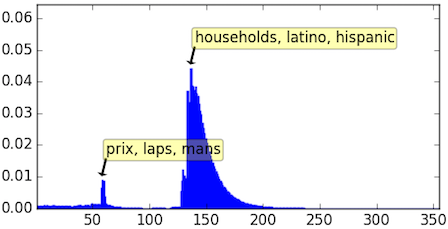
\includegraphics[width=.99\linewidth]{p_z_race.png}
  \caption{$p(z|w=\text{`race'})$}
  \label{fig:sub1p}
\end{subfigure}
\begin{subfigure}{.49\textwidth}
  \centering
  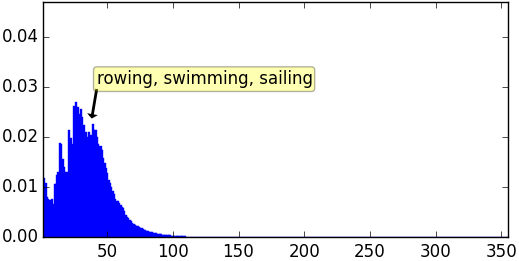
\includegraphics[width=.99\linewidth]{p_z_w_for_regatta.png}
  \caption{$p(z|w=\text{`regatta'})$}
  \label{fig:sub2p}
\end{subfigure}
\begin{subfigure}{.49\textwidth}
  \centering
  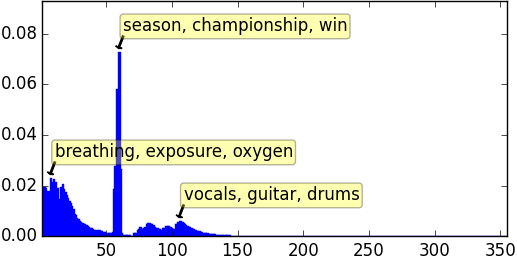
\includegraphics[width=.99\linewidth]{p_z_w_for_lead.png}
  \caption{$p(z|w=\text{`lead'})$}
  \label{fig:sub3p}
\end{subfigure}
\begin{subfigure}{.49\textwidth}
  \centering
  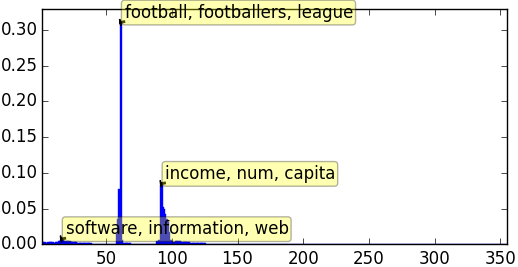
\includegraphics[width=.99\linewidth]{p_z_w_for_net.png}
  \caption{$p(z|w=\text{`net'})$}
  \label{fig:sub4p}
\end{subfigure}
\caption{The four plots above show $p(z|w)$ for the words \textit{race} (a), \textit{regatta} (b), \textit{lead} (c), and \textit{net} (d).  We see the homographs (a, c, d) have more complicated distributions (more modes, probability mass at larger dimensions) than the specific word \textit{regatta}.  This suggests iSG is adapting capacity as expected.}
\label{p_z_plots}
\end{figure}
\section{Evaluation}\label{eval}
We now evaluate our Infinite Skip-Gram (iSG) model qualitatively and quantitatively against original Skip-Gram (SG).  For all experiments, iSG and SG were trained on a one billion word subset of Wikipedia (6/29/08 snapshot).  Three SG models with dimensionalities 100, 300, and 500 were trained with the Word2Vec implementation.  Nine iSG models were trained using combinations of $a = \{1.1, 1.075, 1.05 \}$ and $\lambda = \{ 1\times 10^{-4}, 1\times 10^{-6}, 1\times 10^{-8} \}$, eaching taking approximately twelve hours on a c3.8XL Amazon EC2 instance using thirty threads.  The same learning rate ($\alpha = 0.05$), decay schedule for $\alpha$ (Word2Vec default), number of negative samples (5), context window size (10), and number of training epochs (1) were used for SG and iSG.  iSG was initialized to two dimensions for every run and produced vectors of lengths ranging from 275 to 536 dimensions.  We attempted to use AdaGrad, but experiments showed it made vectors grow to extreme lengths. 
\subsection{Qualitative Results}\label{qual_results}
We begin evaluation by examining the qualitative properties of the embeddings learned by iSG.  We selected four homographs--\textit{bank}, \textit{race}, \textit{net}, and \textit{lead}--to see if iSG can capture their various facets of meaning.  We present nearest neighbor results for the first three and visualize $p(z|w)$ for the last three.  
\subsubsection{Nearest Neighbors}
As has become standard practice when presenting an embedding model, we show that nearest neighbors in the learnt space are semantically related.  Table \ref{nearest} contains the five nearest neighbors for the words \textit{race}, \textit{net}, and \textit{bank} learned by SG and iSG (calculated by Equations \ref{w2v_sim} and \ref{iw2v_sim2} respectively).  The ten nearest neighbors for the same words can be found in Table \ref{nearest_appendix} in the appendix.  The leftmost column shows iSG-produced neighbors when using full marginalization to compute the expected inner product.  The second and third columns show neighbors when approximate marginalization is used to surface different senses of each word.  Original SG's neighbors are in the fourth column.  Comparing iSG's first-column neighbors to SG's, we see that they are all but indistinguishable in the case of \textit{bank}, but neighbors are much different for \textit{race} and \textit{net}.  iSG seems to have found terms related to the biological sense of \textit{race} as the most globally similar while SG finds car racing terms exclusively.  For \textit{net}, SG has only learned an internet-related meaning, but iSG's global results include a mixture of sporting (\textit{goals, liga}) and financial/numerical (\textit{income, score}) terms.  

While perhaps original SG's neighbors are slightly more focused than iSG's first-column neighbors, we see quite conspicuously that SG has failed to recognize that these words are homographs.  That is, SG only captures one meaning in its representation.  Conversely, iSG was able to capture various meanings, which is made clear by the second and third columns of Table \ref{nearest} in which the similarities were calculated by summing over the five words in italic (ex: \textit{car, driver, track, speed, motor}) when computing $p(z|w)$.  Quite dramatically different senses are able to be found through this simple modification, including the senses found by SG.  Furthermore, we find that iSG's vectors are robust to marginalizing with improper contexts.  For instance, calculating \textit{race}'s nearest neighbors by marginalizing over \textit{investment, banking, loan, savings, investment} results in the following five nearest neighbors: \textit{laps, racing, lap, ferrari, prix}.  No banking-related terms were found that, if present, would suggest spurious semantic relationships could be induced by arbitrary choices of words.  
\subsubsection{Modes of Meaning}
Next we show iSG's potential for meaning disambiguation by plotting $p(z|w)$ for the selected homographs and the word \textit{regatta} (from our example in the Introduction); see Figure \ref{p_z_plots}.  The yellow boxes contain the three nearest neighbors as determined by inner product computed over the dimensionality specified by the arrow.  

We see that, as expected, \textit{race} (a) exhibits a much more complicated distribution over dimensions than \textit{regatta} (b) does.  $p(z|w=\text{`race'})$ features at least two prominent modes corresponding to \textit{automobile} and \textit{biological} meanings.  $p(z|w=\text{`regatta'})$ is clearly uni-modal, concentrating around its only meaning (boat race).  Moreover, \textit{race} is a longer vector in the sense that it puts probability mass on as many as 200 dimensions.  \textit{regatta}, on the other hand, has no perceptible probability mass after 100 dimensions. 

We see similarly interesting distributions from the two other homographs plotted, \textit{lead} (c) and \textit{net} (d).  The former appears to have three strong modes corresponding to \textit{lead poisoning}, \textit{leader of a sports team or statistical category}, and \textit{leader in a band} (ex: `lead trumpet').  The latter also has three distinct modes evoking technology, sports, and numerical meanings.  The technology mode is hard to see in Figure \ref{p_z_plots}, but magnifying will reveal a clear plateau.  Notice too the scale of the plot is different than the others due to the dominant middle mode.  And lastly, note that the sports sense common to all words--\textit{prix} in (a), \textit{rowing} in (b), \textit{season} in (c), and \textit{football} in (d)--occurs at roughly the same place in each distribution, at slightly above 50 dimensions.
\subsection{Experiment: Context Prediction}
%We next turn to quantitative evaluation.
\begin{figure}
  \begin{minipage}[c]{0.30\textwidth}
    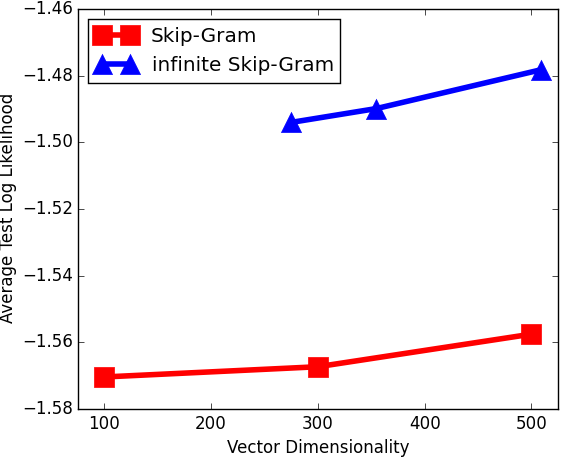
\includegraphics[width=.89\linewidth]{prediction_plt.png}
  \end{minipage}\hfill
  \begin{minipage}[c]{0.70\textwidth}
    \caption{Context prediction.  This Figure shows the average test log likelihood for iSG (blue) and SG (red) at three different vector dimensionalities.  Since the vector length of iSG cannot be specified, models with vectors closest in size to 100, 300, and 500 dimensions were chosen.  iSG vectors had lengths 275, 355, and 509.  iSG is clearly better at predicting context words \emph{despite having the same number of parameters as SG}.} \label{pred_plot}
  \end{minipage}
\end{figure}
%\subsubsection{Context Prediction}
We compared the ability of SG and iSG to predict the context of a given word on a held out test set, which was created from the last thirty-two million words of the same Wikipedia snapshot.  In Figure \ref{pred_plot} we plot the average log likelihood computed by SG (i.e. $\frac{1}{|(w_{i}, c_{k})|} \sum_{(w_{i}, c_{k})} \log p(c_{k} | w_{i})$) with vectors of dimensionality 100, 300, 500 against the iSG average complete-data log likelihood (i.e. $\frac{1}{|(w_{i}, c_{k})|} \sum_{(w_{i}, c_{k})} \log \sum_{z} p(c_{k}, z | w_{i})$) for 275, 355, and 509 dimensional vectors.  These vectors were chosen because their sizes were most comparable to the SG vector dimensionalities.  Notice that even though SG and iSG \emph{have almost exactly the same number of parameters}, iSG has a conspicuously higher log likelihood. 
%\subsubsection{Semantic Similarity}
% moved to end of document

\section{Conclusions and Future Work}
We've proposed a novel word embedding model called \textit{Infinite Skip-Gram} that defines vector dimensionality as a random variable with a countably infinite domain.  Training via the Monte Carlo gradient proposed in Section \ref{learn_isg} allows embeddings to grow as the data requires.  This property is especially well suited for learning representations of homographs--which Skip-Gram notably fails at--and this is demonstrated in Section \ref{qual_results}.  A unique quality of the iSG is that it is highly interpretable (in comparison to other embedding methods) due to its ability to produce a distribution over the dimensionality of a given word ($p(z|w)$).  Plots of $p(z|w)$ such as the ones in Figure \ref{p_z_plots} concisely show how specific/vague a word is and its various senses just from the mode landscape.  Soon we will add more experimental results on word similarity and sense induction tasks.

%\section*{Acknowledgments}
\bibliography{iclr2016_conference}
\bibliographystyle{iclr2016_conference}
\clearpage

\section*{Appendix}
\subsection*{Finite Partition Function}
Below we show that summing over $z \in [1, \infty)$, as needs to be done to calculate the partition function, results in a finite value by way of a convergent geometric series.
\begin{equation*}\begin{split}\label{z_finite_full}
Z_{z} &= \sum_{z=1}^{\infty} e^{-E(\mathbf{w}, \mathbf{c}, z)} \\ &= \sum_{z=1}^{l} e^{-E(\mathbf{w}, \mathbf{c}, z)} + \sum_{z=l+1}^{\infty} e^{-E(\mathbf{w}, \mathbf{c}, z)} \\ &= \sum_{z=1}^{l} e^{-E(\mathbf{w}, \mathbf{c}, z)} + \sum_{z=l+1}^{\infty} e^{-E(\mathbf{w}, \mathbf{c}, l) - (z-l-1)\log a + \sum_{i=l+1}^{z} w_{i}c_{i} - w_{i}^{2} - c_{i}^{2}} \\ &= \sum_{z=1}^{l} e^{-E(\mathbf{w}, \mathbf{c}, z)} + e^{-E(\mathbf{w}, \mathbf{c}, l)} \sum_{z=l+1}^{\infty} e^{  -(z-l-1)\log a + \sum_{i=l+1}^{z} w_{i}c_{i} - w_{i}^{2} - c_{i}^{2} }   \\ &= \sum_{z=1}^{l} e^{-E(\mathbf{w}, \mathbf{c}, z)} + e^{-E(\mathbf{w}, \mathbf{c}, l)} \sum_{z=l+1}^{\infty} e^{  -(z-l-1) \log a } \\ &= \sum_{z=1}^{l} e^{-E(\mathbf{w}, \mathbf{c}, z)} + e^{-E(\mathbf{w}, \mathbf{c}, l)} \sum_{z=0}^{\infty} e^{  -z \log a } \\ &= \sum_{z=1}^{l} e^{-E(\mathbf{w}, \mathbf{c}, z)} + e^{-E(\mathbf{w}, \mathbf{c}, l)} \sum_{z=0}^{\infty} \frac{1}{a^{  z }} \\ &= \sum_{z=1}^{l} e^{-E(\mathbf{w}, \mathbf{c}, z)} + \frac{a}{a-1}e^{-E(\mathbf{w}, \mathbf{c}, l)}.
\end{split}
\end{equation*} 

\subsection*{Finite Expectation}
Next we show that the iSG objective--specifically the expectation over $p(z|w)$ needed for its calculation--is finite.  Again we use the argument that every word and context vector has non-zero elements only up to and including some index $l$.  
\begin{equation*}\begin{split}\label{expectation_full}
\mathbb{E}_{z|w}[- \log p( c_{k}| w_{i}, z)] &= - \sum_{z=1}^{\infty} p(z | w_{i}) \log p(c_{k}| w_{i}, z) \\ &=  - \sum_{z=1}^{l} p(z | w_{i}) \log p(c_{k}| w_{i}, z) +  - \sum_{z=l+1}^{\infty} p(z | w_{i}) \log p(c_{k}| w_{i}, z) .\end{split}\end{equation*}  Clearly the first term is finite, and thus we turn our attention exclusively to the second term: \begin{equation*}\begin{split}\label{expectation_full2}
\sum_{z=l+1}^{\infty} p(z | w_{i}) \log p(c_{k}| w_{i}, z) &= \sum_{z=l+1}^{\infty} p(z | w_{i}) \log \left[ \frac{e^{-E(\mathbf{w}_{i}, \mathbf{c}_{k}, z)}}{ \sum_{\mathbf{c}'} e^{-E(\mathbf{w}_{i}, \mathbf{c}', z)} }  \right]  \\
&= \sum_{z=l+1}^{\infty} p(z | w_{i}) \log \left[ \frac{e^{-E(\mathbf{w}_{i}, \mathbf{c}_{k}, l) - (z-l-1)\log a + \sum_{j=l+1}^{z} w_{i,j}c_{k,j} - w_{i,j}^{2} - c_{k,j}^{2}}}{ \sum_{\mathbf{c}'} e^{-E(\mathbf{w}_{i}, \mathbf{c}', l) - (z-l-1)\log a + \sum_{j=l+1}^{z} w_{i,j}c_{j}' - w_{i,j}^{2} - {c'}_{j}^{2}} }  \right]  \\ 
&= \sum_{z=l+1}^{\infty} p(z | w_{i}) \log \left[ \frac{e^{-E(\mathbf{w}_{i}, \mathbf{c}_{k}, l) - (z-l-1)\log a }}{ \sum_{\mathbf{c}'} e^{-E(\mathbf{w}_{i}, \mathbf{c}', l) - (z-l-1)\log a } }  \right]  \\ 
&= \sum_{z=l+1}^{\infty} p(z | w_{i}) \log \left[ \frac{e^{- (z-l-1)\log a }e^{-E(\mathbf{w}_{i}, \mathbf{c}_{k}, l)}}{ e^{- (z-l-1)\log a }\sum_{\mathbf{c}'} e^{-E(\mathbf{w}_{i}, \mathbf{c}', l)  } }  \right]  \\ 
&= \log p(c_{k}| w_{i}, l) \sum_{z=l+1}^{\infty} p(z | w_{i})  \\ 
&= \log p(c_{k}| w_{i}, l) \frac{1}{Z_{\mathbf{c},z}} \sum_{z=l+1}^{\infty} \sum_{\mathbf{c}'}e^{-E(\mathbf{w}_{i}, \mathbf{c}', z)}  \\ 
&= \log p(c_{k}| w_{i}, l) \frac{1}{Z_{\mathbf{c},z}}  \sum_{\mathbf{c}'}e^{-E(\mathbf{w}_{i}, \mathbf{c}', l)} \sum_{z=l+1}^{\infty} e^{- (z-l-1)\log a }  \\ 
&= \frac{a}{a-1} p(z = l | w_{i})\log p(c_{k}| w_{i}, l) .
\end{split}\end{equation*}  Combining this result with the summation over the first $l$ terms, we see the expectation's analytical form is \begin{equation*}\label{expectation_final}
\mathbb{E}_{z|w}[- \log p( c_{k}| w_{i}, z)] =  - \sum_{z=1}^{l} p(z | w_{i}) \log p(c_{k}| w_{i}, z) +  \frac{-a}{a-1} p(z = l | w_{i})\log p(c_{k}| w_{i}, l) .\end{equation*}

\clearpage
\begin{table}[]
\centering
\begin{tabular}{@{}lll | l@{}}
 \toprule
 \multicolumn{3}{c}{Infinite Skip-Gram (iSG)} & \multicolumn{1}{c}{Skip-Gram (SG)}  \\ \midrule \midrule  \multicolumn{4}{c}{\textbf{race}}              \\  \midrule \midrule
 \multicolumn{1}{c}{full vocabulary} & \multicolumn{1}{c}{\textit{\begin{tabular}[c]{@{}c@{}}car, driver, track, \\ speed, motor\end{tabular}}} & \multicolumn{1}{c}{\textit{\begin{tabular}[c]{@{}c@{}}politics, election, vote,\\ washington, campaign\end{tabular}}} & \multicolumn{1}{c}{n/a}   \\ \midrule
 households  & laps & election  & races  \\ 
 latino      & races   & elections & racing  \\ 
 couples     & busch  & electoral & prix \\ 
 hispanic    & prix  & party     & finish  \\ 
 asian       & nascar  & seats  & drivers  \\ 
 races       & drivers  & senate & driver \\ 
 islander    & lap & republican & pole \\ 
 census      & racing & parliment & standings \\ 
 laps        & ferrari  & democratic & driving \\ 
 population  & asian  & elected   & qualifying \\ 
 
 \midrule \midrule  \multicolumn{4}{c}{\textbf{net}}              \\
  \midrule \midrule \multicolumn{1}{c}{\begin{tabular}[c]{@{}c@{}}full vocabulary\end{tabular}} & \multicolumn{1}{c}{\textit{\begin{tabular}[c]{@{}c@{}}goal, score, win,\\ soccer, hockey\end{tabular}}} & \multicolumn{1}{c}{\textit{\begin{tabular}[c]{@{}c@{}}web, email, online,\\ technology, website\end{tabular}}} & \multicolumn{1}{c}{n/a}     \\ \midrule
 num           & football     & www & com  \\ 
 score         & footballers    & http  & www  \\ 
 income        & nfl       & php & homepage \\ 
 goals         & league              & com & http  \\ 
 liga          & fc     & https      & html   \\ 
 avg      & nhl      & html        & htm  \\ 
 midfielder         & baseball    & index      & asp \\ 
  gross   & hockey              & web & web  \\ 
 yards         & basketball          & org & website  \\ 
 nhl         & rugby               & software   & links \\ 
 \midrule \midrule  \multicolumn{4}{c}{\textbf{bank}}              \\  \midrule \midrule
  \multicolumn{1}{c}{\begin{tabular}[c]{@{}c@{}}full vocabulary\end{tabular}} & \multicolumn{1}{c}{\textit{\begin{tabular}[c]{@{}c@{}}money, finance, loan, \\ savings, investment\end{tabular}}} & \multicolumn{1}{c}{\textit{\begin{tabular}[c]{@{}c@{}}river, stream, water, \\ shore, sand\end{tabular}}} & \multicolumn{1}{c}{n/a}  \\ \midrule
investment    & investment                    & river                 & banks  \\ 
banking       & banking                       & railway               & investment   \\ 
securities    & securities                    & road                  & financial   \\ 
 corporation   & corporation                   & avenue                & insurance  \\ 
 holdings      & currency                      & highway               & finance   \\ 
currency      & dollar & situated              & capital  \\ 
capital       & holdings                      & located               & trading  \\ 
dollar        & saudi & lake                  & exchange  \\ 
owned         & capital                       & bridge                & fund   \\ 
finance       & investors                     & street                & credit  \\ 
\bottomrule
\end{tabular}
\caption{Nearest Neighbors.  The table above is an expanded version of Table \ref{nearest}, displaying the ten nearest neighbors for \textit{race}, \textit{net}, and \textit{bank} as learned by Infinite Skip-Gram (left three columns, retrieved via Equation \ref{iw2v_sim2}) and original Skip-Gram (rightmost column, retrieved via Equation \ref{w2v_sim}).}
\label{nearest_appendix}
\end{table}
\end{document}

\subsection*{Training}
Lastly, we provide a detailed description of the training procedure, including gradient derivations.
\subsubsection*{Preliminaries}
The data necessary to process one training example is a $(V+1)$-sized collection of word tokens $\{w_i, c_{v=1}, \ldots, c_{v=k}, \ldots, c_{v=V_{c}} \}$ where $w_{i}$ is a (center / input) word of current focus, $c_{v}$ is a context word, and $c_{k}$ is a context word observed to appear within a $(K-1)$-sized window around $w_{i}$ in a corpus $\mathcal{D}$.  From this data we'll look to calculate two probabilities.  The first is the conditional probability of the observed context word $c_{k}$ given input word $w_{i}$:
\begin{align*}
p(c_k | w_i, z) = \frac{p(c_k, w_i, z)}{p(w_i, z)} 
= \frac{p(c_k, w_i, z)}{\sum_{v=1}^{V_c} p(c_v, w_i, z)} 
= \frac{e^{-E(\mathbf{w}_i, \mathbf{c}_k,  z)}}{\sum_{v=1}^{V_c} e^{-E( \mathbf{w}_i, \mathbf{c}_v, z)}}.\end{align*}
The second is the conditional probability of the dimensionality $z$ given $w_{i}$:
\begin{align*}
p(z | w_i) = \frac{p(z, w_i)}{p(w_i)} 
= \frac{\sum_{v=1}^{V_c} p(c_v, w_i, z)}
{\sum_{z=1}^{\infty} \sum_{v=1}^{V_c} p(c_v, w_i, z)} = \frac{\sum_{v=1}^{V_c} e^{-E(\mathbf{w}_i, \mathbf{c}_v, z)}}
{\sum_{z=1}^{\infty} \sum_{v=1}^{V_c} e^{-E( \mathbf{w}_i, \mathbf{c}_v, z)}}. 
\end{align*}  See above for the closed-form of $\sum_{z=1}^{\infty} e^{-E( \mathbf{w}_i, \mathbf{c}_v, z)}$.

\subsection*{Efficient Approximations}
Notice that $p(c_k | w_i, z)$ and $p(z | w_i)$ require sums over $V_{c}$, the full context vocabulary, and as a result are expensive to compute.  To alleviate runtime costs, we'll only sum over a subset of the context words; this procedure is known as \textit{negative sampling}.  To compute the sum when it appears in the denominator (normalization constant), we'll gather $S$ negative samples and sum over them.  Hence, we approximate $p(c_k | w_i, z)$ as follows: \begin{align*}
p(c_k | w_i, z)  \approx \frac{e^{-E(\mathbf{w}_i, \mathbf{c}_k,  z)}}{\sum_{s=1}^{S} e^{-E( \mathbf{w}_i, \mathbf{c}_s, z)} + e^{-E( \mathbf{w}_i, \mathbf{c}_k, z)}}.\end{align*}  When the sum appears in the numerator, we'll approximate it slightly differently.  We'll sum over the current context window in order to reduce the variance of $p(z|w)$.  That is, we'll calculate $p(z|w_{i})$ as \begin{align*}
p(z | w_i) \approx \frac{\sum_{i-K\le k \le i+K, k\ne i} e^{-E(\mathbf{w}_i, \mathbf{c}_k, z)} + \sum_{s=1}^{S} e^{-E(\mathbf{w}_i, \mathbf{c}_s, z)}}
{\sum_{z=1}^{\infty} \sum_{i-K\le k \le i+K, k\ne i} e^{-E( \mathbf{w}_i, \mathbf{c}_k, z)} + \sum_{s=1}^{S} e^{-E( \mathbf{w}_i, \mathbf{c}_s, z)}}.\end{align*} 

In addition to the two above, we'll have to employ one more approximation by sampling $z$ in order to compute $\nabla_{\mathbf{w}} \mathcal{L}_{iSG}$ (gradient of Equation \ref{expectation}), despite its analytical form.  The reasons for doing so are described in Section \ref{learn_isg}.  Below we derive the Monte Carlo gradient suggested by \cite{xu2015show}:
\begin{align*}\frac{\partial \mathcal{L}_{iSG}}{\partial \mathbf{w}_{i}} &= 
 \sum_{z=1}^{l} p(z |  \mathbf{w}_i)
\frac{\partial \log p(\mathbf{c}_k  |  \mathbf{w}_i , z)}{\partial \mathbf{w}_{i}}+\frac{\partial p( z  |  \mathbf{w}_i)}{\partial \mathbf{w}_{i}} \log p(\mathbf{c}_k  |  \mathbf{w}_i , z)  \\
&+ \frac{a}{a-1}   p(l  |  \mathbf{w}_i)
\frac{\partial \log p(\mathbf{c}_k  |  \mathbf{w}_i , l)}{\partial \mathbf{w}_{i}} +
\frac{a}{a-1}\frac{\partial p(l |  \mathbf{w}_{i})}{\partial \mathbf{w}_{i}} \log p(\mathbf{c}_{k}  |  \mathbf{w}_{i} , l) \\ 
&=  \sum_{z=1}^{l} p(z |  \mathbf{w}_i)
\frac{\partial \log p(\mathbf{c}_k  |  \mathbf{w}_i , z)}{\partial \mathbf{w}_{i}}+p( z  |  \mathbf{w}_i)\frac{\partial \log p( z  |  \mathbf{w}_i)}{\partial \mathbf{w}_{i}} \log p(\mathbf{c}_k  |  \mathbf{w}_i , z)  \\
&+ \frac{a}{a-1}   p(l  |  \mathbf{w}_i)
\frac{\partial \log p(\mathbf{c}_k  |  \mathbf{w}_i , l)}{\partial \mathbf{w}_{i}} +
\frac{a}{a-1}p(l |  \mathbf{w}_{i}) \frac{\partial \log p(l |  \mathbf{w}_{i})}{\partial \mathbf{w}_{i}} \log p(\mathbf{c}_{k}  |  \mathbf{w}_{i} , l) \\ 
&=  \sum_{z=1}^{l} p(z |  \mathbf{w}_i)
\left[ \frac{\partial \log p(\mathbf{c}_k  |  \mathbf{w}_i , z)}{\partial \mathbf{w}_{i}}+\frac{\partial \log p( z  |  \mathbf{w}_i)}{\partial \mathbf{w}_{i}} \log p(\mathbf{c}_k  |  \mathbf{w}_i , z) \right]  \\
&+ \frac{a}{a-1}   p(l  |  \mathbf{w}_i) \left [
\frac{\partial \log p(\mathbf{c}_k  |  \mathbf{w}_i , l)}{\partial \mathbf{w}_{i}} +
 \frac{\partial \log p(l |  \mathbf{w}_{i})}{\partial \mathbf{w}_{i}} \log p(\mathbf{c}_{k}  |  \mathbf{w}_{i} , l) \right] \\ 
 &\approx \frac{1}{M}  \sum_{m=1}^{M} \frac{\partial \log p(\mathbf{c}_k  |  \mathbf{w}_i , \hat{z}_{m})}{\partial \mathbf{w}_{i}}+\frac{\partial \log p( \hat{z}_{m}  |  \mathbf{w}_i)}{\partial \mathbf{w}_{i}} \log p(\mathbf{c}_k  |  \mathbf{w}_i , \hat{z}_{m}).
\end{align*}  Note that $\hat{z}_{m} = l$ if $l+1$ is sampled. 

\subsubsection*{Gradient Derivation}
Now we'll write-out the Monte Carlo gradients of $\nabla_{\mathbf{w}} \mathcal{L}_{iSG}$ and $\nabla_{\mathbf{c}} \mathcal{L}_{iSG}$ in detail (in that order).  

First let's consider
\begin{align*}\frac{\partial \log p(\mathbf{c}_k  |  \mathbf{w}_i , \hat{z}_{m})}{\partial \mathbf{w}_{i}} &= \frac{\partial}{\partial \mathbf{w}_{i}} \left[ \mathbf{w}_{i}^{T}\mathbf{c}_{k}\Bigr|_{\hat z_{m}} - \| \mathbf{w}_{i} \|_{2}^{2}\Bigr|_{\hat z_{m}}  - \| \mathbf{c}_{k} \|_{2}^{2}\Bigr|_{\hat z_{m}} - \hat z_{m} \log a - \log \sum_{\mathbf{c}_{v}} e^{-E(\mathbf{w}_{i}, \mathbf{c}_{k}, \hat z_{m})}  \right] \\
&= \mathbf{c}_{k}\Bigr|_{\hat z_{m}} - 2\mathbf{w}_{i}\Bigr|_{\hat z_{m}} - \frac{1}{Z_{\mathbf{c}}} \sum_{\mathbf{c}_{v}} e^{-E(\mathbf{w}_{i}, \mathbf{c}_{k}, \hat z_{m})} (\mathbf{c}_{v} - 2\mathbf{w}_{i}) \Bigr|_{\hat z_{m}} \\
&= (\mathbf{c}_{k} - 2\mathbf{w}_{i})\Bigr|_{\hat z_{m}} - p(\mathbf{c}_k  |  \mathbf{w}_i , \hat{z}_m)(\mathbf{c}_{k} - 2\mathbf{w}_{i})\Bigr|_{\hat z_{m}} - \sum_{\mathbf{c}_{v} \setminus \{ \mathbf{c}_{k} \}} p(\mathbf{c}_v  |  \mathbf{w}_i , \hat{z}_m) (\mathbf{c}_{v} - 2\mathbf{w}_{i}) \Bigr|_{\hat z_{m}} \\
&= (1 - p(\mathbf{c}_k  |  \mathbf{w}_i , \hat{z}_m))(\mathbf{c}_{k} - 2\mathbf{w}_{i})\Bigr|_{\hat z_{m}} - \sum_{\mathbf{c}_{v} \setminus \{ \mathbf{c}_{k} \}} p(\mathbf{c}_v  |  \mathbf{w}_i , \hat{z}_m) (\mathbf{c}_{v} - 2\mathbf{w}_{i}) \Bigr|_{\hat z_{m}}.
\end{align*}
Next let's consider
\begin{align*}\frac{\partial \log p(\hat z_{m}  |  \mathbf{w}_i )}{\partial \mathbf{w}_{i}} &= \frac{\partial}{\partial \mathbf{w}_{i}} \log \frac{\sum_{\mathbf{c}_{v}} e^{-E(\mathbf{w}_{i}, \mathbf{c}_{v}, \hat z_{m})}}{Z_{\mathbf{c},z}} \\ &= \frac{\partial}{\partial \mathbf{w}_{i}} \log \sum_{\mathbf{c}_{v}} e^{-E(\mathbf{w}_{i}, \mathbf{c}_{v}, \hat z_{m})} - \log \sum_{\mathbf{c}_{v}}\sum_{z=1}^{\infty} e^{-E(\mathbf{w}_{i}, \mathbf{c}_{v}, z)}\\
 &= \frac{\partial}{\partial \mathbf{w}_{i}} \log \left[ \sum_{\mathbf{c}_{v}} e^{-E(\mathbf{w}_{i}, \mathbf{c}_{v}, \hat z_{m})} \right] - \log \left[ \sum_{\mathbf{c}_{v}}\sum_{z=1}^{l-1} e^{-E(\mathbf{w}_{i}, \mathbf{c}_{v}, z)} + \frac{2a-1}{a-1}\sum_{\mathbf{c}_{v}} e^{-E(\mathbf{w}_{i}, \mathbf{c}_{v}, l)} \right] \\
 &= \frac{1}{Z_{\mathbf{c}}} \sum_{\mathbf{c}_{v}} e^{-E(\mathbf{w}_{i}, \mathbf{c}_{v}, \hat z_{m})} (\mathbf{c}_{v} - 2\mathbf{w}_{i}) \Bigr|_{\hat z_{m}} \\ &- \frac{1}{Z_{\mathbf{c}, z}} \left[ \sum_{\mathbf{c}_{v}}\sum_{z=1}^{l-1} e^{-E(\mathbf{w}_{i}, \mathbf{c}_{v}, z)} (\mathbf{c}_{v} - 2\mathbf{w}_{i}) \Bigr|_{ z}  + \frac{2a-1}{a-1}\sum_{\mathbf{c}_{v}} e^{-E(\mathbf{w}_{i}, \mathbf{c}_{v}, l)} (\mathbf{c}_{v} - 2\mathbf{w}_{i}) \Bigr|_{l} \right] \\
  &=  \sum_{\mathbf{c}_{v}} p( \mathbf{c}_{v} | \mathbf{w}_{i}, \hat z_{m}) (\mathbf{c}_{v} - 2\mathbf{w}_{i}) \Bigr|_{\hat z_{m}} \\ &- \sum_{\mathbf{c}_{v}}\sum_{z=1}^{l-1} p(\mathbf{c}_{v}, z | \mathbf{w}_{i}) (\mathbf{c}_{v} - 2\mathbf{w}_{i}) \Bigr|_{z}  - \frac{2a-1}{a-1}\sum_{\mathbf{c}_{v}} p(\mathbf{c}_{v}, l | \mathbf{w}_{i}) (\mathbf{c}_{v} - 2\mathbf{w}_{i}) \Bigr|_{l}.  \\
\end{align*}
To get a clear picture of the gradient, we need to combine the terms where $\hat z_{m} = z$.  The first case we need to consider is $\hat z_{m} < l$: \begin{align*} &=  \sum_{\mathbf{c}_{v}} p( \mathbf{c}_{v} | \mathbf{w}_{i}, \hat z_{m}) (\mathbf{c}_{v} - 2\mathbf{w}_{i}) \Bigr|_{\hat z_{m}} - \sum_{\mathbf{c}_{v}} p(\mathbf{c}_{v}, \hat{z}_{m} | \mathbf{w}_{i}) (\mathbf{c}_{v} - 2\mathbf{w}_{i}) \Bigr|_{\hat{z}_{m}} \\ &- \sum_{z=1, z \ne \hat{z}_{m}}^{l-1} \sum_{\mathbf{c}_{v}} p(\mathbf{c}_{v}, z | \mathbf{w}_{i}) (\mathbf{c}_{v} - 2\mathbf{w}_{i}) \Bigr|_{z}  - \frac{2a-1}{a-1}\sum_{\mathbf{c}_{v}} p(\mathbf{c}_{v}, l | \mathbf{w}_{i}) (\mathbf{c}_{v} - 2\mathbf{w}_{i}) \Bigr|_{l} \\
&=  \sum_{\mathbf{c}_{v}} p( \mathbf{c}_{v} | \mathbf{w}_{i}, \hat z_{m}) (\mathbf{c}_{v} - 2\mathbf{w}_{i}) \Bigr|_{\hat z_{m}} - p(\hat{z}_{m} | \mathbf{w}_{i})\sum_{\mathbf{c}_{v}} p(\mathbf{c}_{v} | \mathbf{w}_{i}, \hat{z}_{m}) (\mathbf{c}_{v} - 2\mathbf{w}_{i}) \Bigr|_{\hat{z}_{m}} \\ &- \sum_{z=1, z \ne \hat{z}_{m}}^{l-1} p(z | \mathbf{w}_{i}) \sum_{\mathbf{c}_{v}} p(\mathbf{c}_{v} | \mathbf{w}_{i}, z) (\mathbf{c}_{v} - 2\mathbf{w}_{i}) \Bigr|_{z}  - \frac{2a-1}{a-1} p(l | \mathbf{w}_{i} )\sum_{\mathbf{c}_{v}} p(\mathbf{c}_{v} | \mathbf{w}_{i}, l) (\mathbf{c}_{v} - 2\mathbf{w}_{i}) \Bigr|_{l} \\
&=  (1 - p(\hat{z}_{m} | \mathbf{w}_{i})) \sum_{\mathbf{c}_{v}} p(\mathbf{c}_{v} | \mathbf{w}_{i}, \hat{z}_{m}) (\mathbf{c}_{v} - 2\mathbf{w}_{i}) \Bigr|_{\hat{z}_{m}} \\ &- \sum_{z=1, z \ne \hat{z}_{m}}^{l-1} p(z | \mathbf{w}_{i}) \sum_{\mathbf{c}_{v}} p(\mathbf{c}_{v} | \mathbf{w}_{i}, z) (\mathbf{c}_{v} - 2\mathbf{w}_{i}) \Bigr|_{z}  - \frac{2a-1}{a-1} p(l | \mathbf{w}_{i} )\sum_{\mathbf{c}_{v}} p(\mathbf{c}_{v} | \mathbf{w}_{i}, l) (\mathbf{c}_{v} - 2\mathbf{w}_{i}) \Bigr|_{l}.
\end{align*}
The second case occurs when $\hat z_{m} = l$: \begin{align*} &=  \sum_{\mathbf{c}_{v}} p( \mathbf{c}_{v} | \mathbf{w}_{i}, l) (\mathbf{c}_{v} - 2\mathbf{w}_{i}) \Bigr|_{l}  \\ &- \sum_{z=1}^{l-1} p(z | \mathbf{w}_{i})\sum_{\mathbf{c}_{v}} p(\mathbf{c}_{v} | \mathbf{w}_{i}, z) (\mathbf{c}_{v} - 2\mathbf{w}_{i}) \Bigr|_{z}  - \frac{2a-1}{a-1} p(l | \mathbf{w}_{i}) \sum_{\mathbf{c}_{v}} p(\mathbf{c}_{v} | \mathbf{w}_{i}, l) (\mathbf{c}_{v} - 2\mathbf{w}_{i}) \Bigr|_{l} \\
&=  (1 - \frac{2a-1}{a-1} p(l | \mathbf{w}_{i}) ) \sum_{\mathbf{c}_{v}} p( \mathbf{c}_{v} | \mathbf{w}_{i}, l) (\mathbf{c}_{v} - 2\mathbf{w}_{i}) \Bigr|_{l}  - \sum_{z=1}^{l-1} p(z | \mathbf{w}_{i})\sum_{\mathbf{c}_{v}} p(\mathbf{c}_{v} | \mathbf{w}_{i}, z) (\mathbf{c}_{v} - 2\mathbf{w}_{i}) \Bigr|_{z} .
\end{align*}

Now we'll derive the gradient with respect to the \textit{positive} context vector.  First, let's consider 
\begin{align*}\frac{\partial \log p(\mathbf{c}_k  |  \mathbf{w}_i , \hat{z}_{m})}{\partial \mathbf{c}_{k}} &= \frac{\partial}{\partial \mathbf{c}_{k}} \left[ \mathbf{w}_{i}^{T}\mathbf{c}_{k}\Bigr|_{\hat z_{m}} - \| \mathbf{w}_{i} \|_{2}^{2}\Bigr|_{\hat z_{m}}  - \| \mathbf{c}_{k} \|_{2}^{2}\Bigr|_{\hat z_{m}} - \hat z_{m} \log a - \log \sum_{\mathbf{c}_{v}} e^{-E(\mathbf{w}_{i}, \mathbf{c}_{v}, \hat z_{m})}  \right] \\
&= \mathbf{w}_{i}\Bigr|_{\hat z_{m}} - 2\mathbf{c}_{k}\Bigr|_{\hat z_{m}} - \frac{1}{Z_{\mathbf{c}}} e^{-E(\mathbf{w}_{i}, \mathbf{c}_{k}, \hat z_{m})} (\mathbf{w}_{i} - 2\mathbf{c}_{k}) \Bigr|_{\hat z_{m}} \\
&= (1 - p(c_{k} | w_{i}, z)) (\mathbf{w}_{i} - 2\mathbf{c}_{k})\Bigr|_{\hat z_{m}} 
\end{align*}

Next we'll derive the gradient with respect to the \textit{negative} context vector:
\begin{align*}\frac{\partial \log p(\mathbf{c}_k  |  \mathbf{w}_i , \hat{z}_{m})}{\partial \mathbf{c}_{v}} &= \frac{\partial}{\partial \mathbf{c}_{v}} \left[ \mathbf{w}_{i}^{T}\mathbf{c}_{k}\Bigr|_{\hat z_{m}} - \| \mathbf{w}_{i} \|_{2}^{2}\Bigr|_{\hat z_{m}}  - \| \mathbf{c}_{k} \|_{2}^{2}\Bigr|_{\hat z_{m}} - \hat z_{m} \log a - \log \sum_{\mathbf{c}_{v}} e^{-E(\mathbf{w}_{i}, \mathbf{c}_{v}, \hat z_{m})}  \right] \\
&=  -\frac{1}{Z_{\mathbf{c}}} e^{-E(\mathbf{w}_{i}, \mathbf{c}_{v}, \hat z_{m})} (\mathbf{w}_{i} - 2\mathbf{c}_{v}) \Bigr|_{\hat z_{m}} \\
&= -p(c_{v} | w_{i}, z) (\mathbf{w}_{i} - 2\mathbf{c}_{v})\Bigr|_{\hat z_{m}} 
\end{align*}

Now we'll find the gradient of $\log p(z | w_{i})$ with respect to a context vector:
\begin{align*}\frac{\partial \log p(\hat z_{m}  |  \mathbf{w}_i )}{\partial \mathbf{c}_{v}} &= \frac{\partial}{\partial \mathbf{c}_{v}} \log \frac{\sum_{\mathbf{c}_{v}} e^{-E(\mathbf{w}_{i}, \mathbf{c}_{v}, \hat z_{m})}}{Z_{\mathbf{c},z}} \\ &= \frac{\partial}{\partial \mathbf{c}_{v}} \log \sum_{\mathbf{c}_{v}} e^{-E(\mathbf{w}_{i}, \mathbf{c}_{v}, \hat z_{m})} - \log \sum_{\mathbf{c}_{v}}\sum_{z=1}^{\infty} e^{-E(\mathbf{w}_{i}, \mathbf{c}_{v}, z)}\\
 &= \frac{\partial}{\partial \mathbf{c}_{v}} \log \left[ \sum_{\mathbf{c}_{v}} e^{-E(\mathbf{w}_{i}, \mathbf{c}_{v}, \hat z_{m})} \right] - \log \left[ \sum_{\mathbf{c}_{v}}\sum_{z=1}^{l-1} e^{-E(\mathbf{w}_{i}, \mathbf{c}_{v}, z)} + \frac{2a-1}{a-1}\sum_{\mathbf{c}_{v}} e^{-E(\mathbf{w}_{i}, \mathbf{c}_{v}, l)} \right] \\
 &= \frac{1}{Z_{\mathbf{c}}} e^{-E(\mathbf{w}_{i}, \mathbf{c}_{v}, \hat z_{m})} (\mathbf{w}_{i} - 2\mathbf{c}_{v}) \Bigr|_{\hat z_{m}} \\ &- \frac{1}{Z_{\mathbf{c}, z}} \left[ \sum_{z=1}^{l-1} e^{-E(\mathbf{w}_{i}, \mathbf{c}_{v}, z)} (\mathbf{w}_{i} - 2\mathbf{c}_{v}) \Bigr|_{ z}  + \frac{2a-1}{a-1} e^{-E(\mathbf{w}_{i}, \mathbf{c}_{v}, l)} (\mathbf{w}_{i} - 2\mathbf{c}_{v}) \Bigr|_{l} \right] \\
  &=  p( \mathbf{c}_{v} | \mathbf{w}_{i}, \hat z_{m}) (\mathbf{w}_{i} - 2\mathbf{c}_{v}) \Bigr|_{\hat z_{m}} \\ &- \sum_{z=1}^{l-1} p(\mathbf{c}_{v}, z | \mathbf{w}_{i}) (\mathbf{w}_{i} - 2\mathbf{c}_{v}) \Bigr|_{z}  - \frac{2a-1}{a-1} p(\mathbf{c}_{v}, l | \mathbf{w}_{i}) (\mathbf{w}_{i} - 2\mathbf{c}_{v}) \Bigr|_{l} \\
  &=  p( \mathbf{c}_{v} | \mathbf{w}_{i}, \hat z_{m}) (\mathbf{w}_{i} - 2\mathbf{c}_{v}) \Bigr|_{\hat z_{m}} \\ &- \sum_{z=1}^{l-1} p(z | w_{i}) p(\mathbf{c}_{v} | \mathbf{w}_{i}, z) (\mathbf{w}_{i} - 2\mathbf{c}_{v}) \Bigr|_{z}  - \frac{2a-1}{a-1}p(l | w_{i}) p(\mathbf{c}_{v} | \mathbf{w}_{i}, l) (\mathbf{w}_{i} - 2\mathbf{c}_{v}) \Bigr|_{l}.
\end{align*}
Again, we'll consider the gradient when $\hat{z}_{m} < l$ and when $\hat{z}_{m} = l$.  In the former case: \begin{align*}  &=  (1 - p(\hat{z}_{m} | w_{i})) p( \mathbf{c}_{v} | \mathbf{w}_{i}, \hat z_{m}) (\mathbf{w}_{i} - 2\mathbf{c}_{v}) \Bigr|_{\hat z_{m}} \\ &- \sum_{z=1, z \ne \hat{z}_{m} }^{l-1} p(z | w_{i}) p(\mathbf{c}_{v} | \mathbf{w}_{i}, z) (\mathbf{w}_{i} - 2\mathbf{c}_{v}) \Bigr|_{z}  - \frac{2a-1}{a-1}p(l | w_{i}) p(\mathbf{c}_{v} | \mathbf{w}_{i}, l) (\mathbf{w}_{i} - 2\mathbf{c}_{v}) \Bigr|_{l} .
\end{align*}  And in the latter case we have:
\begin{align*}  &=  (1 - \frac{2a-1}{a-1}p(l | w_{i})) p( \mathbf{c}_{v} | \mathbf{w}_{i}, l) (\mathbf{w}_{i} - 2\mathbf{c}_{v}) \Bigr|_{l} - \sum_{z=1 }^{l-1} p(z | w_{i}) p(\mathbf{c}_{v} | \mathbf{w}_{i}, z) (\mathbf{w}_{i} - 2\mathbf{c}_{v}) \Bigr|_{z}  .
\end{align*}

To summarize, above we have derived the following five gradients.  We'll write them below with respect to individual elements for clarity.

\begin{align*}\frac{\partial \log p(\mathbf{c}_k  |  \mathbf{w}_i , \hat{z}_{m})}{\partial w_{i,j}} &= (c_{k,j} - 2w_{i,j}) - \sum_{\mathbf{c}_{v}}p(c_{v} | w_{i}, \hat{z}_{m}) (c_{v,j} - 2w_{i,j}). \end{align*} 

\begin{align*}\frac{\partial \log p(\mathbf{c}_k  |  \mathbf{w}_i , \hat{z}_{m})}{\partial c_{v,j}} &= (\mathbbm{1}_{v = k} - p(c_{k} | w_{i}, \hat{z}_{m} )) (w_{i,j} - 2c_{k,j}). \end{align*} 

\begin{align*}\frac{\partial \log p(\hat z_{m}  |  \mathbf{w}_i )}{\partial w_{i,j}} &=
  \sum_{\mathbf{c}_{v}} p( c_{v} | w_{i}, \hat z_{m}) (c_{v,j} - 2w_{i,j}) - \sum_{z=j}^{l-1} p(z | w_{i}) \sum_{\mathbf{c}_{v}} p(c_{v} | w_{i}, z) (c_{v,j} - 2w_{i,j}) \\ &- \frac{2a-1}{a-1}p(l|w_{i}) \sum_{\mathbf{c}_{v}} p(c_{v} | w_{i}, l) (c_{v,j} - 2 w_{i,j}). 
\end{align*}

\begin{align*}\frac{\partial \log p(\hat z_{m}  |  \mathbf{w}_i )}{\partial c_{v,j}} &= p( c_{v} | w_{i}, \hat z_{m}) (w_{i,j} - 2c_{v,j}) - \sum_{z=j}^{l-1} p(z | w_{i}) p(c_{v} | w_{i}, z) (w_{i,j} - 2c_{v,j}) \\ &- \frac{2a-1}{a-1}p(l | w_{i}) p(c_{v} | w_{i}, l) (w_{i,j} - 2c_{v,j}).
\end{align*}






%%%% START BLOCK COMMENT %%%% 
\iffalse
And now we'll consider the other needed derivative
\begin{align*}\frac{\partial  p(\hat z_{m}  |  \mathbf{w}_i )}{\partial \mathbf{w}_{i}} &= \frac{\partial}{\partial \mathbf{w}_{i}} \frac{\sum_{\mathbf{c}_{v}} e^{-E(\mathbf{w}_{i}, \mathbf{c}_{v}, \hat z_{m})}}{Z_{\mathbf{c},z}}\\
&=  \frac{\frac{\partial}{\partial \mathbf{w}_{i}} \sum_{\mathbf{c}_{v}} e^{-E(\mathbf{w}_{i}, \mathbf{c}_{v}, \hat z_{m})}}{Z_{\mathbf{c},z}} + \frac{- \sum_{\mathbf{c}_{v}} e^{-E(\mathbf{w}_{i}, \mathbf{c}_{v}, \hat z_{m})}}{Z^{2}_{\mathbf{c},z}} \frac{\partial Z_{\mathbf{c},z}}{\partial \mathbf{w}_{i}} \\
&=  \frac{ \sum_{\mathbf{c}_{v}} e^{-E(\mathbf{w}_{i}, \mathbf{c}_{v}, \hat z_{m})} (\mathbf{c}_{v} - 2\mathbf{w}_{i})\Bigr|_{\hat z_{m}} }{Z_{\mathbf{c},z}} + p(\hat z_{m}  |  \mathbf{w}_i ) \frac{-1}{Z_{\mathbf{c},z}} \frac{\partial Z_{\mathbf{c},z}}{\partial \mathbf{w}_{i}}.
\end{align*}
Focusing on the $\frac{\partial Z_{\mathbf{c},z}}{\partial \mathbf{w}_{i}}$ term we have
\begin{align*}\frac{\partial Z_{\mathbf{c},z}}{\partial \mathbf{w}_{i}} &= \frac{\partial}{\partial \mathbf{w}_{i}} \left[ \sum_{\mathbf{c}_{v}}\sum_{z=1}^{l} e^{-E(\mathbf{w}_{i}, \mathbf{c}_{v}, z)} + \frac{a}{a-1} e^{-E(\mathbf{w}_{i}, \mathbf{c}_{v}, l)} \right] \\ 
&=  \sum_{\mathbf{c}_{v}}\sum_{z=1}^{l} e^{-E(\mathbf{w}_{i}, \mathbf{c}_{v}, z)}(\mathbf{c}_{v} - 2\mathbf{w}_{i})\Bigr|_{z} + \frac{a}{a-1} e^{-E(\mathbf{w}_{i}, \mathbf{c}_{v}, l)}(\mathbf{c}_{v} - 2\mathbf{w}_{i})\Bigr|_{l} \\ 
&=  \sum_{z=1}^{l}\sum_{\mathbf{c}_{v}} e^{-E(\mathbf{w}_{i}, \mathbf{c}_{v}, z)}(\mathbf{c}_{v} - 2\mathbf{w}_{i})\Bigr|_{z} + \sum_{\mathbf{c}_{v}}\frac{a}{a-1} e^{-E(\mathbf{w}_{i}, \mathbf{c}_{v}, l)}(\mathbf{c}_{v} - 2\mathbf{w}_{i})\Bigr|_{l} 
\\ 
&=  \sum_{z=1}^{l-1}\sum_{\mathbf{c}_{v}} e^{-E(\mathbf{w}_{i}, \mathbf{c}_{v}, z)}(\mathbf{c}_{v} - 2\mathbf{w}_{i})\Bigr|_{z} + \frac{2a-1}{a-1}\sum_{\mathbf{c}_{v}}e^{-E(\mathbf{w}_{i}, \mathbf{c}_{v}, l)}(\mathbf{c}_{v} - 2\mathbf{w}_{i})\Bigr|_{l} .
\end{align*}
Now we'll recombine with the full expression, factoring out $1 / Z_{\mathbf{c},z}$:
\begin{align*}\frac{\partial  p(\hat z_{m}  |  \mathbf{w}_i )}{\partial \mathbf{w}_{i}} &= \frac{1}{Z_{\mathbf{c},z}} [ \sum_{\mathbf{c}_{v}} e^{-E(\mathbf{w}_{i}, \mathbf{c}_{v}, \hat z_{m})} (\mathbf{c}_{v} - 2\mathbf{w}_{i})\Bigr|_{\hat z_{m}} \\ &-  p(\hat z_{m}  |  \mathbf{w}_i ) [  \sum_{z=1}^{l-1}\sum_{\mathbf{c}_{v}} e^{-E(\mathbf{w}_{i}, \mathbf{c}_{v}, z)}(\mathbf{c}_{v} - 2\mathbf{w}_{i})\Bigr|_{z} + \frac{2a-1}{a-1}\sum_{\mathbf{c}_{v}}e^{-E(\mathbf{w}_{i}, \mathbf{c}_{v}, l)}(\mathbf{c}_{v} - 2\mathbf{w}_{i})\Bigr|_{l}  ]  ]. \end{align*} 
Next, to get a clear picture of the gradient, we need to combine the terms where $\hat z_{m} = z$.  First, consider when $\hat z_{m} < l$.  In that case we have:
 \begin{align*} = \frac{1}{Z_{\mathbf{c},z}} [ (1 - p(\hat z_{m}  |  \mathbf{w}_i ) )\sum_{\mathbf{c}_{v}} e^{-E(\mathbf{w}_{i}, \mathbf{c}_{v}, \hat z_{m})} (\mathbf{c}_{v} - 2\mathbf{w}_{i})\Bigr|_{\hat z_{m}}  \\ -  p(\hat z_{m}  |  \mathbf{w}_i ) [ \sum_{z=1, z \ne \hat z_{m}}^{l-1}\sum_{\mathbf{c}_{v}} e^{-E(\mathbf{w}_{i}, \mathbf{c}_{v}, z)}(\mathbf{c}_{v} - 2\mathbf{w}_{i})\Bigr|_{z} + \frac{2a-1}{a-1}\sum_{\mathbf{c}_{v}}e^{-E(\mathbf{w}_{i}, \mathbf{c}_{v}, l)}(\mathbf{c}_{v} - 2\mathbf{w}_{i})\Bigr|_{l}  ]  ]. \end{align*}  Then in the case where $\hat z_{m} = l $, we have:
 \begin{align*} = \frac{1}{Z_{\mathbf{c},z}} [ (1 - p( l  |  \mathbf{w}_i )\frac{2a}{a-1} )\sum_{\mathbf{c}_{v}} e^{-E(\mathbf{w}_{i}, \mathbf{c}_{v}, l)} (\mathbf{c}_{v} - 2\mathbf{w}_{i})\Bigr|_{l} -  p(l  |  \mathbf{w}_i ) [ \sum_{z=1}^{l-1}\sum_{\mathbf{c}_{v}} e^{-E(\mathbf{w}_{i}, \mathbf{c}_{v}, z)}(\mathbf{c}_{v} - 2\mathbf{w}_{i})\Bigr|_{z}  ]  ]. \end{align*}  And finally, when the model has chosen to expand (i.e. $\hat z_{m} > l $), we have:
 \begin{align*}= \frac{1}{Z_{\mathbf{c},z}} [  \sum_{\mathbf{c}_{v}} e^{-E(\mathbf{w}_{i}, \mathbf{c}_{v}, l+1)} (\mathbf{c}_{v} - 2\mathbf{w}_{i})\Bigr|_{l+1} -  p(l + 1 |  \mathbf{w}_i ) [ \sum_{z=1}^{l-1}\sum_{\mathbf{c}_{v}} e^{-E(\mathbf{w}_{i}, \mathbf{c}_{v}, z)}(\mathbf{c}_{v} - 2\mathbf{w}_{i})\Bigr|_{z} + \\ \frac{2a-1}{a-1}\sum_{\mathbf{c}_{v}}e^{-E(\mathbf{w}_{i}, \mathbf{c}_{v}, l)}(\mathbf{c}_{v} - 2\mathbf{w}_{i})\Bigr|_{l}  ]  ] .\end{align*}
 For the ultimate step, we'll distribute $1 / Z_{\mathbf{c},z}$ so as to interpret the exponential terms as probabilities.  For $\hat z_{m} < l$ we have
  \begin{align*} =  (1 - p(\hat z_{m}  |  \mathbf{w}_i ) )\sum_{\mathbf{c}_{v}} p(\mathbf{c}_{v}, \hat z_{m} | \mathbf{w}_{i}) (\mathbf{c}_{v} - 2\mathbf{w}_{i})\Bigr|_{\hat z_{m}}  \\ -  p(\hat z_{m}  |  \mathbf{w}_i )  \sum_{z=1, z \ne \hat z_{m}}^{l-1}\sum_{\mathbf{c}_{v}} p(\mathbf{c}_{v}, z | \mathbf{w}_{i}) (\mathbf{c}_{v} - 2\mathbf{w}_{i})\Bigr|_{z} - p(\hat z_{m}  |  \mathbf{w}_i ) \frac{2a-1}{a-1}\sum_{\mathbf{c}_{v}} p(\mathbf{c}_{v}, l | \mathbf{w}_{i}) (\mathbf{c}_{v} - 2\mathbf{w}_{i})\Bigr|_{l}    . \end{align*} 
  For $\hat z_{m} = l$ we have \begin{align*} =  (1 - p( l  |  \mathbf{w}_i )\frac{2a}{a-1} )\sum_{\mathbf{c}_{v}} p(\mathbf{c}_{v}, l | \mathbf{w}_{i}) (\mathbf{c}_{v} - 2\mathbf{w}_{i})\Bigr|_{l} -  p(l  |  \mathbf{w}_i )  \sum_{z=1}^{l-1}\sum_{\mathbf{c}_{v}}p(\mathbf{c}_{v}, z | \mathbf{w}_{i})(\mathbf{c}_{v} - 2\mathbf{w}_{i})\Bigr|_{z} . \end{align*}  
  And finally for $\hat z_{m} > l $ we have \begin{align*}=  \sum_{\mathbf{c}_{v}} p(\mathbf{c}_{v}, l+1 | \mathbf{w}_{i}) (\mathbf{c}_{v} - 2\mathbf{w}_{i})\Bigr|_{l+1} -  p(l + 1 |  \mathbf{w}_i )  \sum_{z=1}^{l-1}\sum_{\mathbf{c}_{v}} p(\mathbf{c}_{v}, z | \mathbf{w}_{i})(\mathbf{c}_{v} - 2\mathbf{w}_{i})\Bigr|_{z} \\ -  p(l + 1 |  \mathbf{w}_i )\frac{2a-1}{a-1}\sum_{\mathbf{c}_{v}}p(\mathbf{c}_{v}, l | \mathbf{w}_{i})(\mathbf{c}_{v} - 2\mathbf{w}_{i})\Bigr|_{l}  .\end{align*}
 \fi
 %%%% END BLOCK COMMENT %%%% 
 


Next we test iSG's ability to rank word pairs according to their semantic similarity, a task commonly used to gauge the quality of embeddings. 

\begin{table}
\centering
\begin{tabular}{l*{6}{c}r}
\bf{Model} & \bf{WordSim-353} & \bf{MEN} \\
\hline
Skip-gram-100d & 0.670 & 0.719 \\
Skip-gram-300d & 0.701 & 0.752 \\
Skip-gram-500d & 0.706 & 0.758 \\
iSG-275d & 0.545 & 0.564 \\ 
iSG-355d & 0.545 & 0.594 \\
iSG-509d & 0.584 & 0.594 \\
\end{tabular}
\quad
\begin{tabular}{l*{6}{c}r}
\bf{Model} & \bf{SCWS} \\
\hline
Skip-gram-100d & 0.637 \\
Skip-gram-300d & 0.659 \\
Skip-gram-500d & 0.660 \\
iSG-275d & 0.536 \\ 
iSG-355d & 0.562 \\
iSG-509d & 0.549 \\
\end{tabular}
\caption{Results on similarity tasks. The numbers are Spearmans correlation between
model's scores and human scores.  The numbers are Spearmans correlation between
model's scores and human scores but are assigned based on 
context in which pair of words is given.}
\end{table}

\subsubsection{Sense Induction}